%Version 3.1 December 2024
% Springer Nature LaTeX Template
\documentclass[pdflatex,sn-mathphys-num]{sn-jnl}% Math and Physical Sciences Numbered Reference Style

%%%% Standard Packages
\usepackage{graphicx}%
\usepackage{multirow}%
\usepackage{amsmath,amssymb,amsfonts}%
\usepackage{amsthm}%
\usepackage{mathrsfs}%
\usepackage[title]{appendix}%
\usepackage{xcolor}%
\usepackage{textcomp}%
\usepackage{manyfoot}%
\usepackage{booktabs}%
\usepackage{algorithm}%
\usepackage{algorithmicx}%
\usepackage{algpseudocode}%
\usepackage{listings}%

%%%% Packages for Dataset Table
\usepackage{longtable}%
\usepackage{array}%
\usepackage{ragged2e}%

\newcolumntype{L}[1]{>{\RaggedRight\arraybackslash}p{#1}}

\raggedbottom

\begin{document}

\title[Deep Learning-Based Kidney Disease Diagnosis: A Comprehensive Survey]{Deep Learning-Based Kidney Disease Diagnosis: A Comprehensive Survey of CT Imaging, Multi-Class Classification, Explainability, and Surgical Planning Frameworks}

%%=============================================================%%
%% Authors and Affiliations                                    %%
%%=============================================================%%

\author*[1]{\fnm{Atharv Ashwin} \sur{Chavan}}\email{2303116@ritindia.edu}

\author[1]{\fnm{Yash Sagar} \sur{Kumbhoje}}\email{2303117@ritindia.edu}

\author[1]{\fnm{Pradnya Ravindra} \sur{Shikalgar}}\email{2303121@ritindia.edu}

\author[1]{\fnm{Kanishka Subhash} \sur{Gavali}}\email{2303122@ritindia.edu}

\author[1]{\fnm{Gautami G.} \sur{Shingan}}

\affil*[1]{\orgdiv{Department of Computer Science \& Engineering}, \orgname{KES's Rajarambapu Institute of Technology}, \orgaddress{\city{Rajaramnagar}, \country{India}}}

%%==================================%%
%% Abstract                         %%
%%==================================%%

\abstract{Kidney diseases present a significant global health challenge, traditionally requiring time-intensive manual interpretation of radiological imaging. Deep learning (DL) has emerged as a transformative approach for the automated diagnosis, segmentation, and prognostic evaluation of renal pathologies. However, existing literature often isolates single tasks, lacking a cohesive review of multi-class classification and surgical planning integration. This survey systematically reviews 63 recent studies focusing on DL applications in kidney disease diagnosis, primarily utilizing CT imaging. We analyze core architectural evolutions, spanning convolutional neural networks (CNNs) to hybrid Transformer models, and evaluate their performance on benchmark datasets. Furthermore, we critically examine the integration of Explainable AI (XAI) and the transition from isolated bounding-box detection to holistic, 3D multimodal clinical frameworks. We identify current research gaps, proposing a unified framework to bridge the gap between computational accuracy and clinical utility.}

%%==================================%%
%% Keywords                         %%
%%==================================%%

\keywords{Deep Learning, Kidney Disease, Computed Tomography (CT), Explainable AI (XAI), Vision Transformers, Surgical Planning}

\maketitle

% --- 1. INTRODUCTION ---
\section{Introduction}
\label{sec:intro}

Kidney diseases, encompassing both neoplastic formations (such as renal cell carcinoma) and non-neoplastic conditions (such as nephrolithiasis and complex cysts), represent a mounting global health challenge. Precise and timely diagnostic workflows are critical for patient survival and effective surgical intervention. Traditionally, the identification, staging, and volumetric analysis of these pathologies have relied almost exclusively on the manual inspection of Computed Tomography (CT) and Magnetic Resonance Imaging (MRI) scans by expert radiologists. This conventional paradigm is inherently subjective, highly time-consuming, and susceptible to inter-observer variability, particularly when differentiating subtle malignant subtypes or delineating complex, multi-focal tumor boundaries for partial nephrectomies.

In recent years, the integration of deep learning (DL) into medical image analysis has fundamentally disrupted this diagnostic bottleneck~\cite{degadwala2024review}. DL architectures, specifically those engineered for advanced computer vision tasks, excel at extracting high-dimensional, non-linear semantic features from complex anatomical structures. While early computational applications in nephrology focused predominantly on binary classification (e.g., normal versus abnormal tissue), the current clinical frontier demands highly granular multi-class classification, exact 3D volumetric segmentation for preoperative planning, and robust algorithmic interpretability. A vast and accelerating body of recent literature has empirically validated the efficacy of these automated approaches across diverse clinical datasets, varying noise profiles, and different stages of disease progression~\cite{aljohani2025hierarchical, obaid2025noisy, khan2025multilevel, verma2025automated, rehman2024kidney, scales2012prevalence, wang2022survival, rajendran2025kidney}.

Despite accelerating algorithmic advancements, a critical translational gap remains between high-performing computational models and their actual deployment in clinical environments. Many contemporary models function as opaque "black boxes"~\cite{kadhim2024machine}, lacking the diagnostic explainability required to build trust among medical practitioners. Furthermore, diagnostic networks are frequently trained on narrow, homogeneous datasets, which severely limits their ability to generalize across diverse clinical hardware and disparate patient demographics.

This survey comprehensively synthesizes the methodologies, computational complexities, and clinical integrations of 63 recent DL frameworks. By meticulously analyzing the trajectory from traditional convolutional networks to advanced hybrid Transformer models, this paper aims to establish a clear taxonomy of current progress. Ultimately, we identify existing structural gaps and chart the necessary trajectory toward clinically viable, explainable AI (XAI) systems that integrate seamlessly into real-world renal care pipelines.

% --- 2. SURVEY METHODOLOGY ---
\section{Survey Methodology}
\label{sec:methodology}

To ensure a rigorous, transparent, and reproducible review of the current landscape, a systematic literature search was conducted following the Preferred Reporting Items for Systematic Reviews and Meta-Analyses (PRISMA) guidelines.

\subsection{Search Strategy and Selection Criteria}
The primary literature search was executed across major scientific databases, including IEEE Xplore, PubMed/MEDLINE, SpringerLink, and arXiv. The search was chronologically restricted to publications from the last five years to capture the most contemporary, state-of-the-art DL architectures. The core Boolean search string utilized combinations of the following keywords: ("Deep Learning" OR "CNN" OR "Transformer" OR "YOLO") AND ("Kidney Disease" OR "Renal Tumor" OR "Kidney Stone") AND ("CT Imaging" OR "Segmentation" OR "Classification" OR "Multi-class").

Initial screening yielded a substantial corpus of preliminary articles. These were subsequently evaluated against strict inclusion criteria: (1) empirical utilization of deep learning models on renal imaging modalities, (2) clear, quantitative reporting of performance metrics (e.g., Accuracy, Dice Similarity Coefficient, Intersection over Union), and (3) direct relevance to multi-class classification, volumetric segmentation, or surgical planning integration. 

\begin{figure}[htbp]
\centering
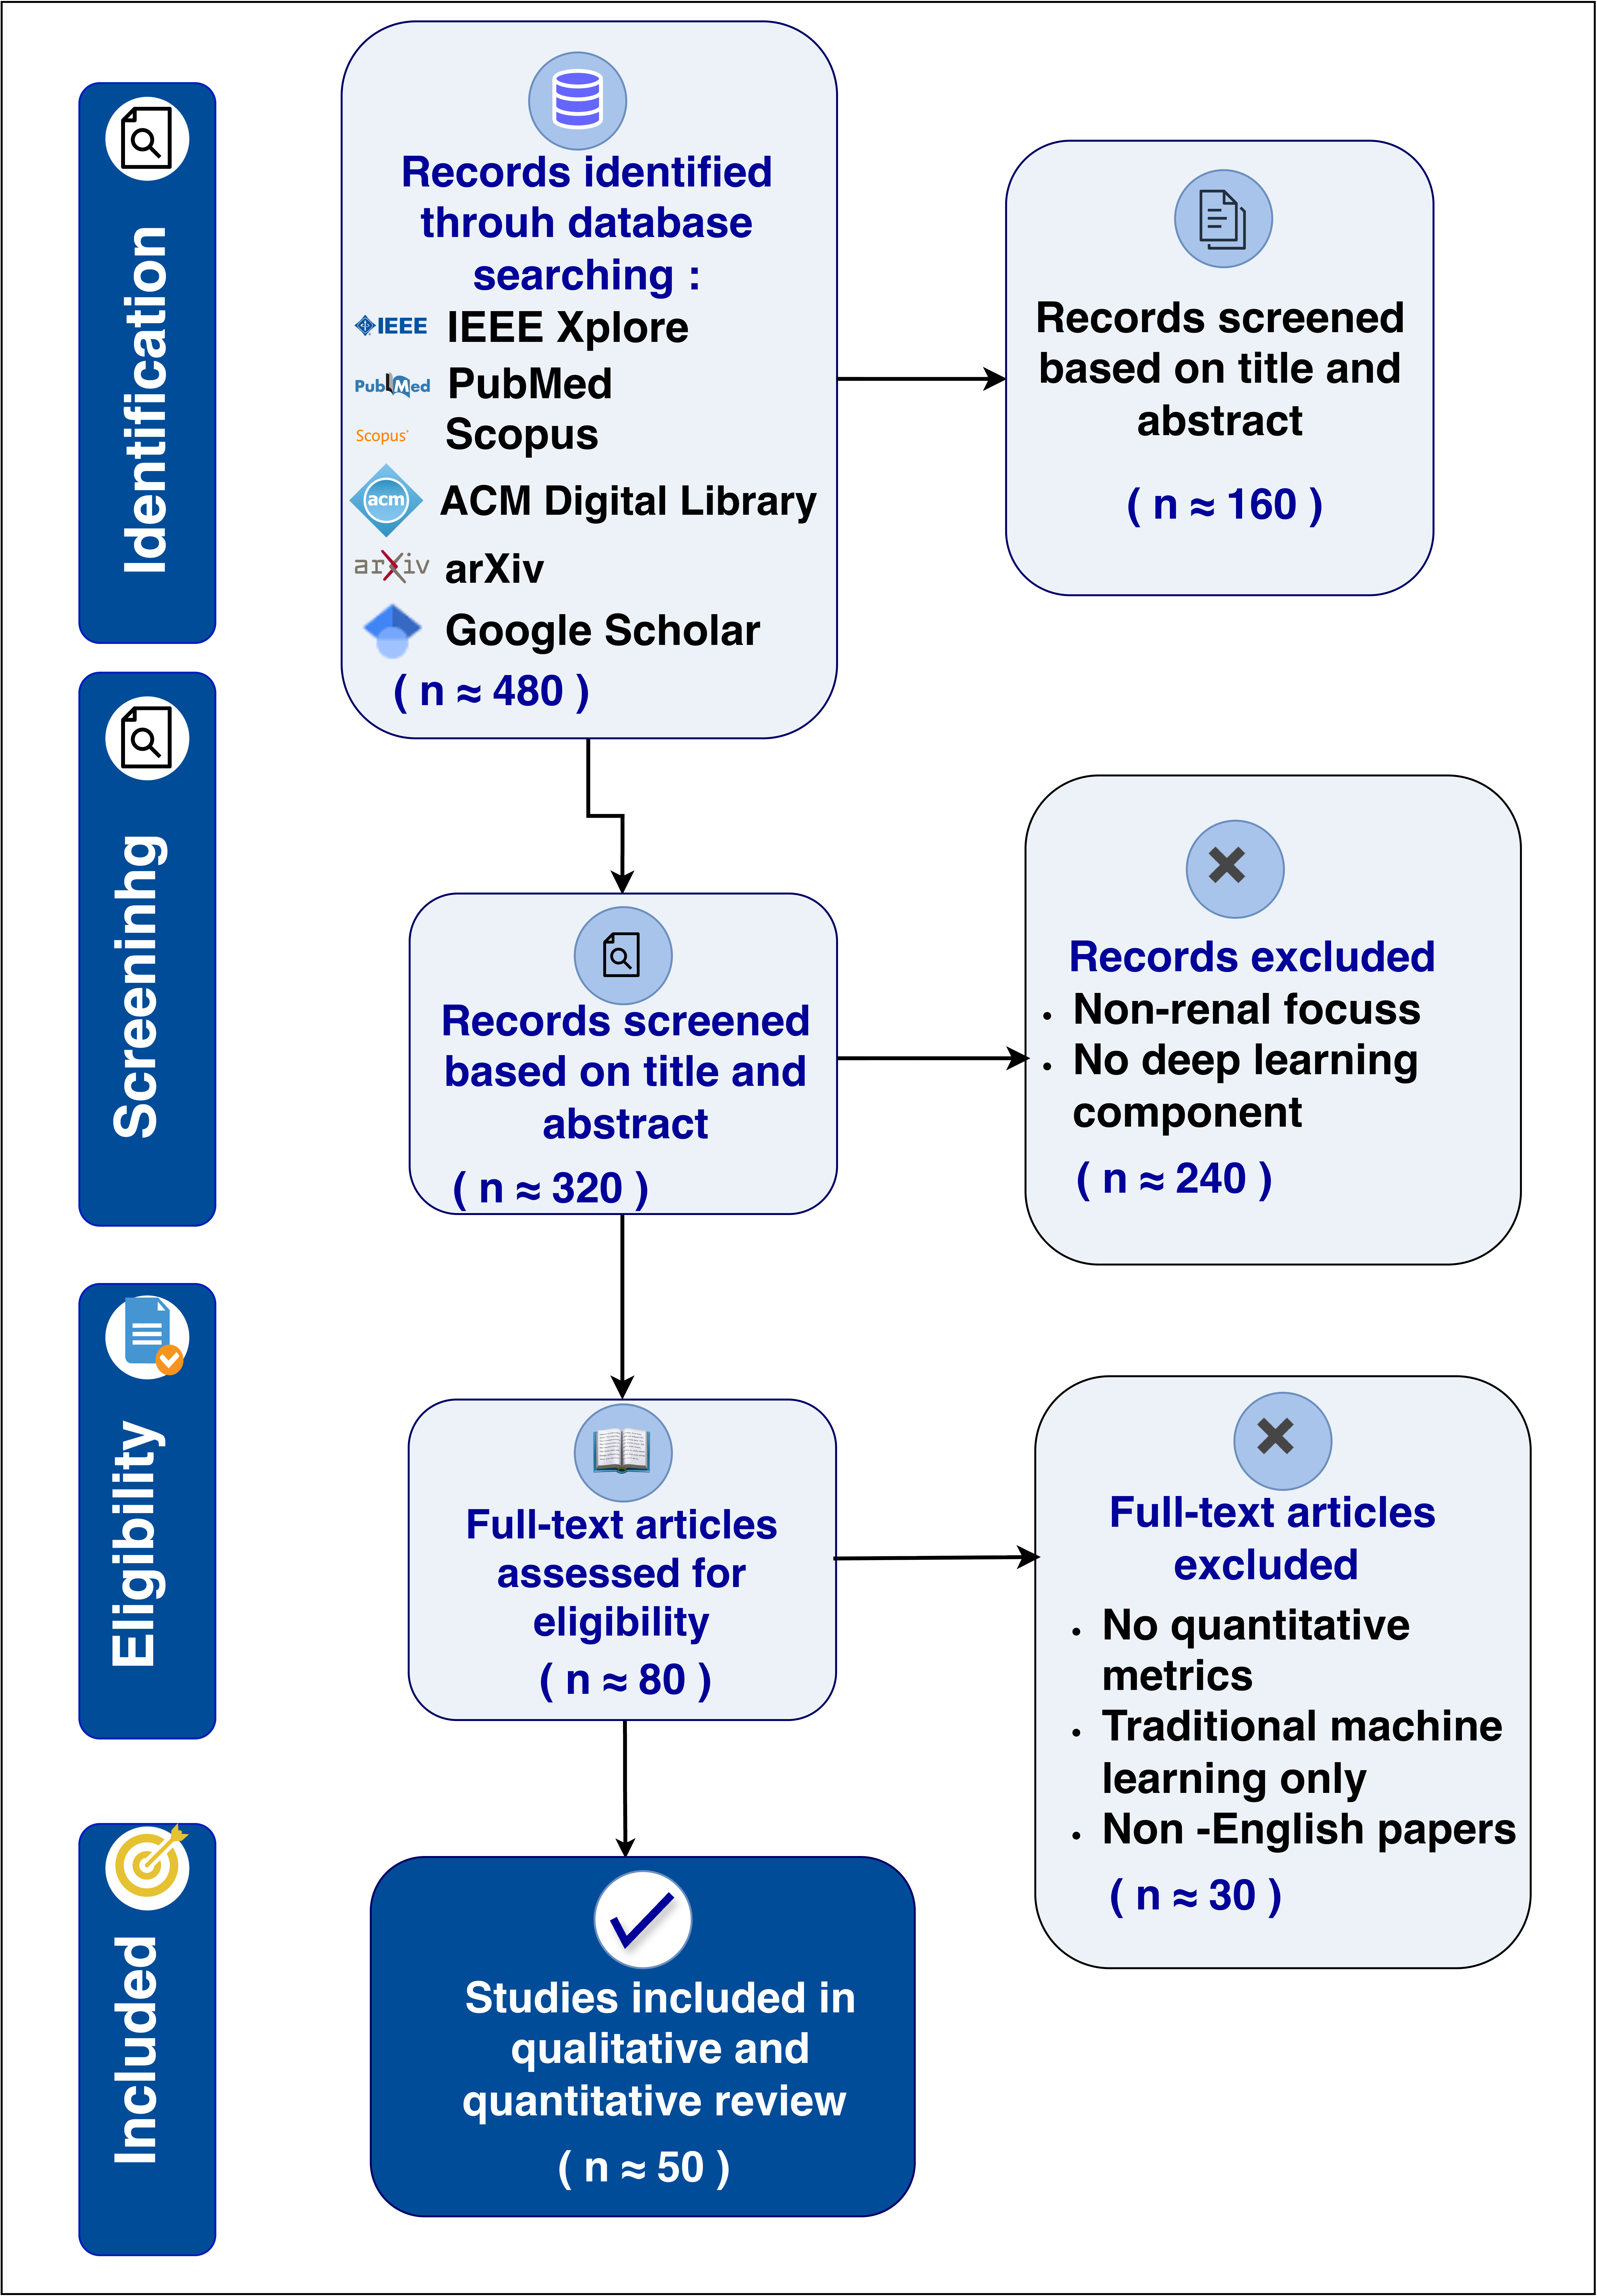
\includegraphics[width=\linewidth]{images/prisma_flow.png}
\caption{PRISMA flow diagram detailing the systematic literature search, screening, and selection process for the 63 included studies.}
\label{fig:prisma}
\end{figure}

\subsection{Data Extraction and Matrix Synthesis}
Following the removal of duplicates, non-peer-reviewed preprints lacking methodological rigor, and studies with insufficient computational detail, 63 primary papers were selected for deep extraction. For each study, data was systematically mapped into a comprehensive literature matrix. The extracted parameters include the imaging modality, primary pathology focus, dataset characteristics (e.g., benchmark challenge data versus proprietary clinical data), core model architecture, computational complexity, integration of Explainable AI (XAI), and identified deployment limitations.

\subsection{Identified Limitations in Current Literature}
Several persistent limitations that delay the seamless translation of computational models into real-world clinical environments are exhibited by the current literature on deep learning (DL) for renal disease diagnosis. In many contemporary architectures, diagnostic explainability is lacking, and these models are often regarded as opaque "black boxes"---a shortcoming that has been identified as a critical barrier to clinical adoption, since the trust of medical practitioners cannot easily be built without it~\cite{kadhim2024machine}.

Furthermore, significant feature limitations are found to persist across various modeling paradigms. In traditional machine learning approaches and hand-crafted feature descriptors (such as GLCM or ALBP), the semantic depth required to navigate the high variability of renal pathologies across diverse patient demographics is not achieved, and high sensitivity to imaging noise and low-resolution scans has been observed~\cite{farjad2021ct, hossain2024adaptive}. Conversely, although lightweight architectures are increasingly prioritized in order to reduce computational overhead and enable rapid, high-throughput triage, a loss of high-level semantic features is sometimes caused by the reduction in network layers in these models, and diagnostic precision is occasionally reduced after highly complex or multi-focal tumor presentations are encountered~\cite{bhandari2023lightweight, alqahtani2025kidneynext}.

Crucially, since narrow, homogeneous repositories are used to train a vast majority of frameworks, poor performance on unseen data is exhibited by several models. Severe performance degradation is frequently suffered when domain shifts are encountered caused by scanner heterogeneity, varying slice thicknesses, and vendor-specific HU calibrations across different hospital networks~\cite{aljohani2025hierarchical, abdelrahman2022deep, alzubi2022kidney, gao2026multitask}. This generalizability deficit is further exacerbated by a widespread lack of prospective clinical verification; in numerous research papers, static, public benchmark datasets are relied upon strictly, and no external multi-center validation or real-world clinical testing is conducted~\cite{liang2025multicenter, hossain2025detection, macin2025kidneynext, chen2023glunet, ye2026automated}.

Finally, single computational tasks---such as classification or segmentation---are frequently isolated by existing diagnostic pipelines, rather than holistic patient metadata and longitudinal clinical history being integrated, and overall utility in complex, real-world decision-making for surgical planning is thereby limited~\cite{liang2025multicenter, sreenivas2025enhancing}.

% --- 3. KEY DATASETS AND BENCHMARKS ---
\clearpage


\section{Key Datasets and Benchmarks}
The evolution of deep learning in renal imaging is intrinsically linked to the availability of large-scale, annotated datasets. Table \ref{tab:datasets} presents a synthesized breakdown of deep learning benchmarks, medical imaging cohorts, and textual corpora utilized across the reviewed literature, grouped categorically by data source. Figure \ref{fig:dataset_dist} illustrates the quantitative distribution of these datasets across the reviewed studies.

% --- Bar Chart Placed Immediately Below the Paragraph ---
\begin{figure}[h!]
\centering
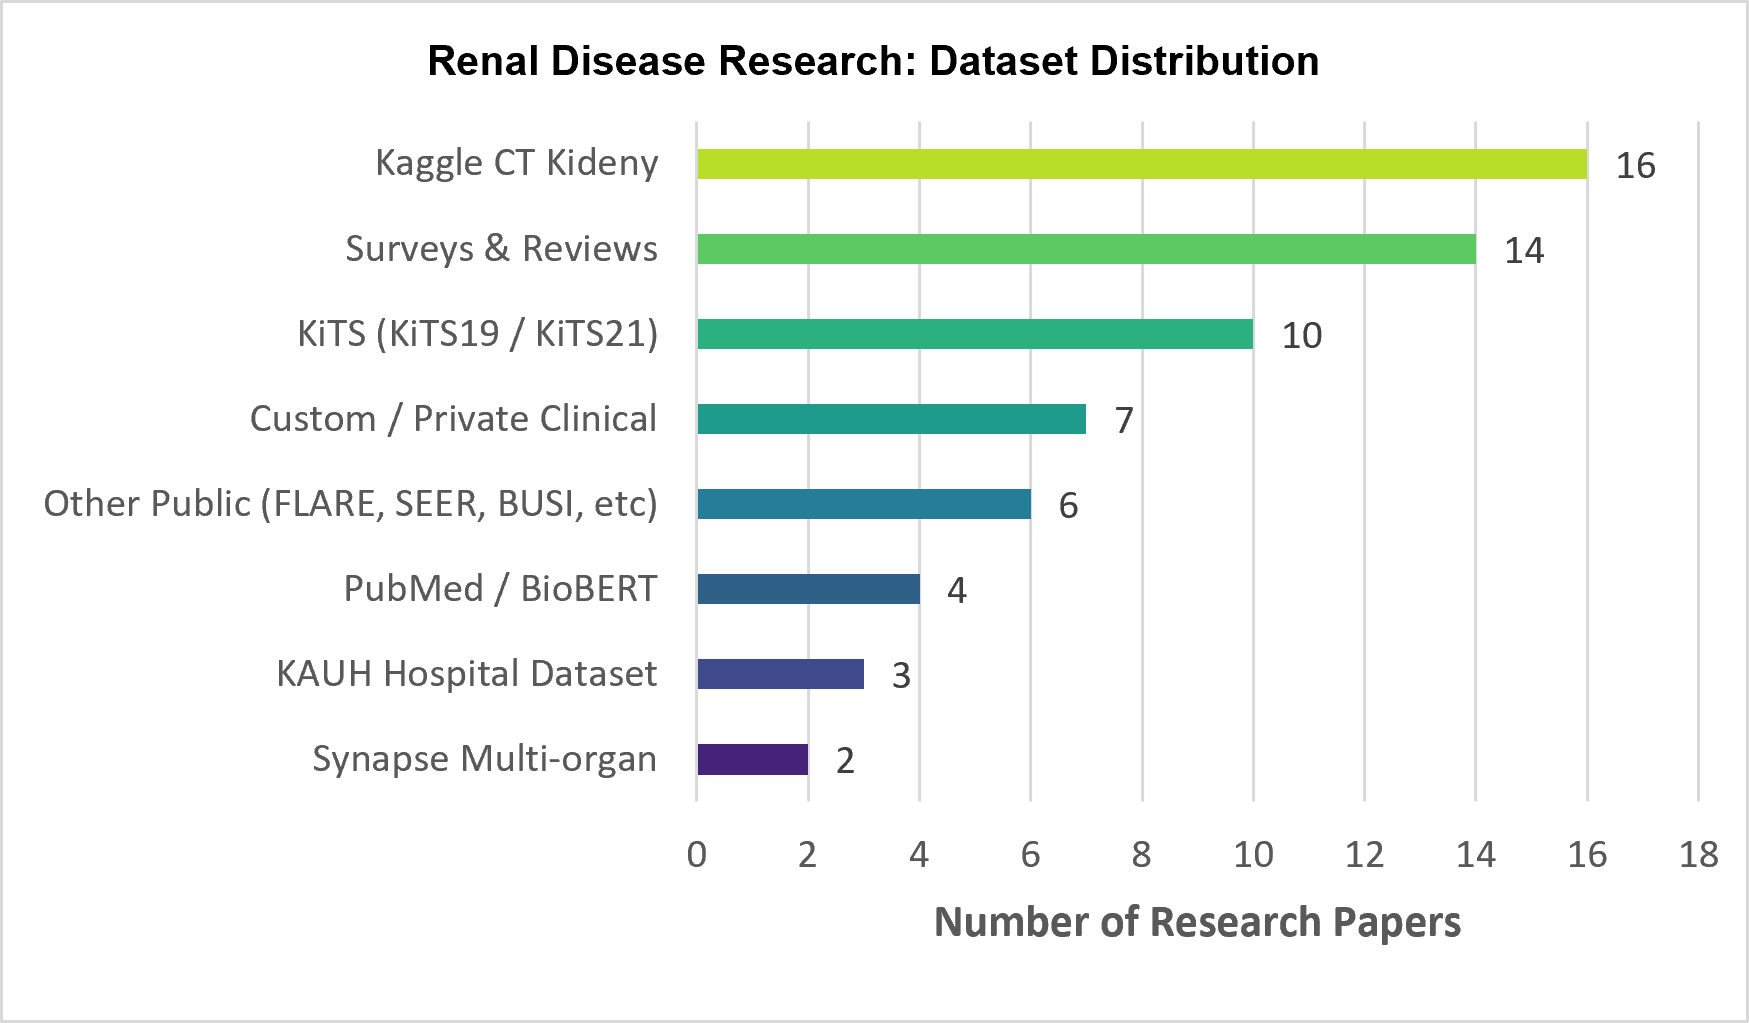
\includegraphics[width=0.85\textwidth]{images/dataset_distribution.png}
\caption{Quantitative distribution of datasets utilized across the reviewed renal disease research papers.}
\label{fig:dataset_dist}
\end{figure}

\vspace{1em} % Adds breathing room between the chart and the table

\renewcommand{\arraystretch}{1.5}  
\setlength{\tabcolsep}{2.5pt}          
\footnotesize                        

\begin{longtable}{|L{2.2cm}|L{1.3cm}|L{1.6cm}|L{2.2cm}|L{2.8cm}|L{1.7cm}|}
\caption{Summary of Reviewed Studies Grouped by Dataset (Papers 1--62)}
\label{tab:datasets} \\
\hline
\textbf{Dataset Name \& Link} & \textbf{Modality} & \textbf{Target Classes} & \textbf{Sample Size \& Breakdown} & \textbf{Performance Highlights} & \textbf{Utilizing Studies} \\
\hline
\endfirsthead

\multicolumn{6}{c}%
{{\bfseries \tablename\ \thetable{} -- continued from previous page}} \\
\hline
\textbf{Dataset Name \& Link} & \textbf{Modality} & \textbf{Target Classes} & \textbf{Sample Size \& Breakdown} & \textbf{Performance Highlights} & \textbf{Utilizing Studies} \\
\hline
\endhead

\hline
\multicolumn{6}{|r|}{{Continued on next page}} \\
\hline
\endfoot

\hline
\endlastfoot

\textbf{\href{https://www.kaggle.com/datasets/nazmul0087/ct-kidney-dataset-normal-cyst-tumor-and-stone}{Kaggle CT Kidney Dataset}} \newline (Dhaka Hospital) & CT (Contrast \& Non-contrast) & Normal, Cyst, Tumor, Stone (4 Classes) & Total: 12,446 images \newline Normal: 5,077 \newline Cyst: 3,709 \newline Tumor: 2,283 \newline Stone: 1,377 & Accuracies ranging from 91.47\% to 99.84\%; F1-scores up to $>0.99$; High diagnostic consistency across CNN and ViT architectures & \cite{khan2025multilevel}, \cite{verma2025automated}, \cite{rajendran2025kidney}, \cite{bhandari2023lightweight}, \cite{rathva2025ensemble}, \cite{tarul2025empirical}, \cite{pimpalkar2025fine}, \cite{alqahtani2025kidneynext}, \cite{islam2022vision}, \cite{sajid2026yolov8}, \cite{alebada2026hybrid}, \cite{hossain2024adaptive}, \cite{sharma2025hybrid}, \cite{martin2025evaluation}, \cite{ahmed2021ct}, \cite{tawfik2026pcsa}, \cite{hossain2025detection}, \cite{macin2025kidneynext} \\
\hline
\textbf{\href{https://github.com/neheller/kits19/tree/master/data}{KiTS19 Challenge}} \newline (Tumor Seg. 2019) & Corticomedullary CT & Kidney, Tumor (2 Seg. Classes) & 300 CT cases total \newline 210 training / 90 testing & Kidney Dice: up to 0.974 \newline Tumor Dice: 0.615 to 0.846 \newline Composite Dice: 0.907 & \cite{ji2024asdnet}, \cite{abdelrahman2023efficientnet}, \cite{hatsutani2023protuberance}, \cite{xie2020seru} \\
\hline
\textbf{\href{https://github.com/neheller/kits21/tree/master/kits21/data}{KiTS21 Challenge}} \newline (Tumor Seg. 2021) & Corticomedullary CT & Kidney, Tumor, Cyst (3 Seg. Classes) & 300 CT cases (Official training cohort with multi-annotator consensus) & Kidney Dice: up to 0.968 \newline Tumor Dice: up to 0.829 \newline Cyst Dice: up to 0.701 & \cite{heller2023kits21}, \cite{gohil2024kidney}, \cite{zhao2023automatic}, \cite{chen20215d} \\
\hline
\textbf{\href{https://www.cancerimagingarchive.net/collection/c4kc-kits/}{C4KC-KiTS}} \newline (Imaging Archive) & CT & 11 Clinical / Anatomical Seg. Classes & Routine clinical nephrectomy scans from heterogeneous institutions & Peak classification and segmentation accuracy up to 99.60\% & \cite{sherryl2022ied} \\
\hline
\textbf{\href{https://www.synapse.org/#!Synapse:syn3193805/wiki/217789}{Synapse Multi-Organ}} \& \textbf{\href{https://flare.grand-challenge.org/Data/}{FLARE Benchmarks}} & Abdominal CT, Dermoscopy, Colonoscopy & Multi-organ abdominal segmentation, skin lesions, polyps & Synapse: 30 CT cases \newline ISIC: 2,694 images \newline CVC-ClinicDB: 612 images & Kidney Dice: 77.8\% to 85.2\% \newline Overall multi-organ Dice up to 85.17\%; IoU up to 84.93\% & \cite{azad2023daeformer}, \cite{lan2024braunet}, \cite{ma2022flare} \\
\hline
\textbf{\href{https://github.com/DaliaAlzubi/KidneyTumor}{KAUH Dataset}} \& Associated CT Sets & CT Scans & Tumor, Normal, Malignant (up to 4 classes) & Total: 8,400 clinical images & Outperformed ResNet50 baselines; Maximum classification accuracy of 98.29\% & \cite{aljohani2025hierarchical}, \cite{alzubi2022kidney} \\
\hline
\textbf{\href{https://universe.roboflow.com/proyecto-1/tesis-iz9ji}{Multi-Center US Repository}} & Ultrasound (US) & Cysts, Stones, Tumors (3 Classes) & $>10,000$ ultrasound frames from multi-center cohorts & Peak F1-score of 0.95 across multi-class detection tasks & \cite{obaid2025noisy} \\
\hline
\textbf{\href{https://www.sciencedirect.com/science/article/pii/S2352340919312181}{BUSI, BUS, \& Dataset B}} & Grayscale B-mode Ultrasound & Benign, Malignant, Normal & BUSI: 780 (487 benign, 210 malignant, 133 normal) \newline Dataset B: 163 & Ultrasound segmentation Dice: 78.69\% to 82.34\%; IoU ranging from 67.94\% to 72.54\% & \cite{he2023h2former} \\
\hline
\textbf{\href{https://zenodo.org/record/6042410}{Zenodo Open-Access Abdominal CT}} & Unenhanced Abdominal CT & Kidney, Kidney Stone, Background & 260 CT scans total \newline 209 with stones / 51 without & Kidney Dice: 96.54\% \newline Stone Dice: 80.59\% \newline Specificity: 99.99\% \newline Stone Sensitivity: 79.73\% & \cite{li2022automatic} \\
\hline
\textbf{\href{https://www.kaggle.com/datasets/orvile/axial-ct-imaging-dataset-kidney-stone-detection}{Sulaimani / Rania Dataset}} & Axial CT & Kidney Stones & 3,364 original axial CT images; expanded to 35,457 via augmentation & High sensitivity and robust feature detection in stone identification frameworks & \cite{abdalla2025axial} \\
\hline
\textbf{\href{https://www.cancerimagingarchive.net/collection/ct-colonography/}{TCIA CT Colonography}} & Non-contrast CT & Kidney Stones & 551 clinical CT scans & Automated detection sensitivity reaching 88.1\% & \cite{elton2022deep} \\
\hline
\textbf{\href{https://www.niddkrepository.org/studies/crisp/}{NIDDK / CRISP Repository}} & MRI (T1 \& T2) & Kidney, Cortex, Medulla (3 Anatomical Classes) & $\sim$241 MRI volumes from multicenter PKD studies & High precision anatomical segmentation: Dice 0.974 (kidney), 0.963 (cortex), 0.950 (medulla) & \cite{raj2022deep} \\
\hline
\textbf{\href{https://www.cdc.gov/nchs/nhanes/index.htm}{NHANES}} \& \textbf{\href{https://seer.cancer.gov/}{SEER Databases}} & Epidemiological Surveys, Proteomics & Kidney Stones (NHANES); Renal Cell Carcinoma (SEER) & NHANES: 12,110 participants \newline SEER: $>22,000$ RCC patient records & NHANES: Stone prevalence 8.8\% \newline SEER: Prognostic AUC of 0.746 for RCC survival models & \cite{scales2012prevalence}, \cite{wang2022survival} \\
\hline
\textbf{\href{https://huggingface.co/datasets/ncbi/pubmed}{Biomedical NLP \& Clinical Text}} & Biomedical Text \& Clinical Notes (NLP) & Symptoms, Diseases, Medications, NER, QA & Up to 14M abstracts / 4.5B words (PubMed/PMC); 300 clinical notes (MACCROBAT) & SOTA performance on biomedical QA and BLURB benchmarks; 86.6\% accuracy on clinical DiRAG tasks & \cite{lee2020biobert}, \cite{fang2023bioformer}, \cite{luo2022biogpt}, \cite{gu2021domain}, \cite{sreenivas2025enhancing} \\
\hline
\textbf{Histopathology} \& \textbf{Urine Microscopy} & Histopathology (H\&E) \& Microscopic Urine & 5 Cancer Grades (Grade 0–4); 14 Urine Particle Classes & Histopathology: 3,000 images \newline Urine Microscopy: 7,201 images & Histopathology: Acc 88.90\%, F1 72.01\% \newline Urine Microscopy: 60\% mAP@50 & \cite{akhtar2026yolov11} \\
\hline

% ---------------------------------------------------------
% SEPARATED PRIVATE DATASETS
% ---------------------------------------------------------

\textbf{Private CT Dataset} \newline (Rehman et al., 2024) & CT & Binary / Multiclass (Stones) & Total: $\sim$5,000 images & Acc: 90–95\% & \cite{rehman2024kidney} \\
\hline
\textbf{Private Multimodal Dataset} \newline (Chen, 2021) & Multimodal (CT / MRI) & Renal masses / tumors & 27 patients & 10.07\% mean abs. diff. & \cite{chen2021rapid} \\
\hline
\textbf{Private Multi-phase CT Dataset} \newline (Liang, 2025) & CT multi-phase & Renal Cell Carcinoma; Urothelial Carcinoma; Urinary Tract Stones & 1024 cases: 326 RCC | 278 urothelial | 420 stones & Dice 90.3\%; IoU 83.6\%; F1 +3.2\% vs EfficientNet-B3 & \cite{liang2025multicenter} \\
\hline
\textbf{Private CT Dataset} \newline (Farjad et al., 2021) & CT & Binary (Normal vs. abnormal) & Total: 150 images (75 normal | 75 abnormal) & Acc: 90\% & \cite{farjad2021ct} \\
\hline
\textbf{Clinical KUB/Fluoroscopy} \newline (Elmaagac et al., 2026) & CT (KUB for PCNL) & Stone-free vs. Non-stone-free outcomes & 340 patients (retrospective clinical study) & AUC: 0.786; Sensitivity: 75\%; Specificity: 76\% & \cite{elmaagac2026comparison} \\
\hline
\textbf{Private KUB X-ray Dataset} \newline (Nguyen et al., 2025) & X-ray (KUB plain film) & Kidney stone detection (binary) & 152 KUB X-rays & YOLOv7-R+CBAM + SR: mAP50 95.0\% & \cite{nguyen2025super} \\
\hline
\textbf{Private Ultrasound Dataset} \newline (Gao et al., 2026) & Ultrasound (grayscale B-mode) & Benign vs. Malignant renal tumor & 345 patients (3,504 images after augmentation) & Segmentation IoU: 94.23\%; Classification AUC: 0.88 & \cite{gao2026multitask} \\
\hline
\textbf{Private Ultrasound Dataset} \newline (Chen et al., 2023) & Ultrasound & Kidney organ, parenchyma, renal sinus & Total: 1,000 images & Dice: 96.25\% (kidney), 92.9\% (parenchyma) & \cite{chen2023glunet} \\
\hline
\textbf{Private CT Dataset} \newline (Ye et al., 2026) & CT & Kidney Stone & Total: 4,000 slices & mAP@0.5: 0.91 & \cite{ye2026automated} \\
\hline
\textbf{Private PACS Dataset} \newline (Noorelahi et al., 2025) & CT / PACS & Radiation dose parameters & 200 patients & Dose variability results & \cite{noorelahi2025pacs} \\
\hline

% ---------------------------------------------------------
% SURVEYS
% ---------------------------------------------------------

\textbf{Survey Papers \& Literature Reviews} \newline (No Primary Experimental Dataset) & Multimodal (CT, MRI, US, X-ray, PET-CT) & N/A (Aggregated review metrics) & Summaries of up to 112+ reviewed articles across various medical imaging domains & Compiles state-of-the-art literature metrics (reported Dice scores up to 0.987 across primary studies) & \cite{degadwala2024review}, \cite{kadhim2024machine}, \cite{abdelrahman2022deep}, \cite{papanastasiou2024systematic} \\
\hline
\end{longtable}



\normalsize

% --- 4. DEEP LEARNING ARCHITECTURES ---
\section{Deep Learning Architectures: A Categorical Review}
\label{sec:architectures}

The computational approach to renal imaging has undergone a significant paradigm shift over the last five years. Early diagnostic automation relied heavily on classical machine learning, utilizing hand-crafted feature extraction methods such as Gray-Level Co-occurrence Matrices (GLCM) paired with Support Vector Machines~\cite{farjad2021ct}. While interpretable, these methods lacked the semantic depth required to navigate the high variability of renal pathologies across diverse patient demographics. 

The advent of deep learning largely replaced these classical pipelines. Based on our systematic review of 63 studies, contemporary architectures can be distinctly categorized by their foundational feature-extraction mechanisms into three evolutionary stages: Convolutional Neural Networks (CNNs), pure Vision Transformers (ViTs), and emerging Hybrid CNN-Transformer frameworks. Figure~\ref{fig:taxonomy} provides a structural taxonomy of these approaches, further subdivided by their primary clinical task and functional mechanisms.

\begin{figure*}[htbp] 
\centering
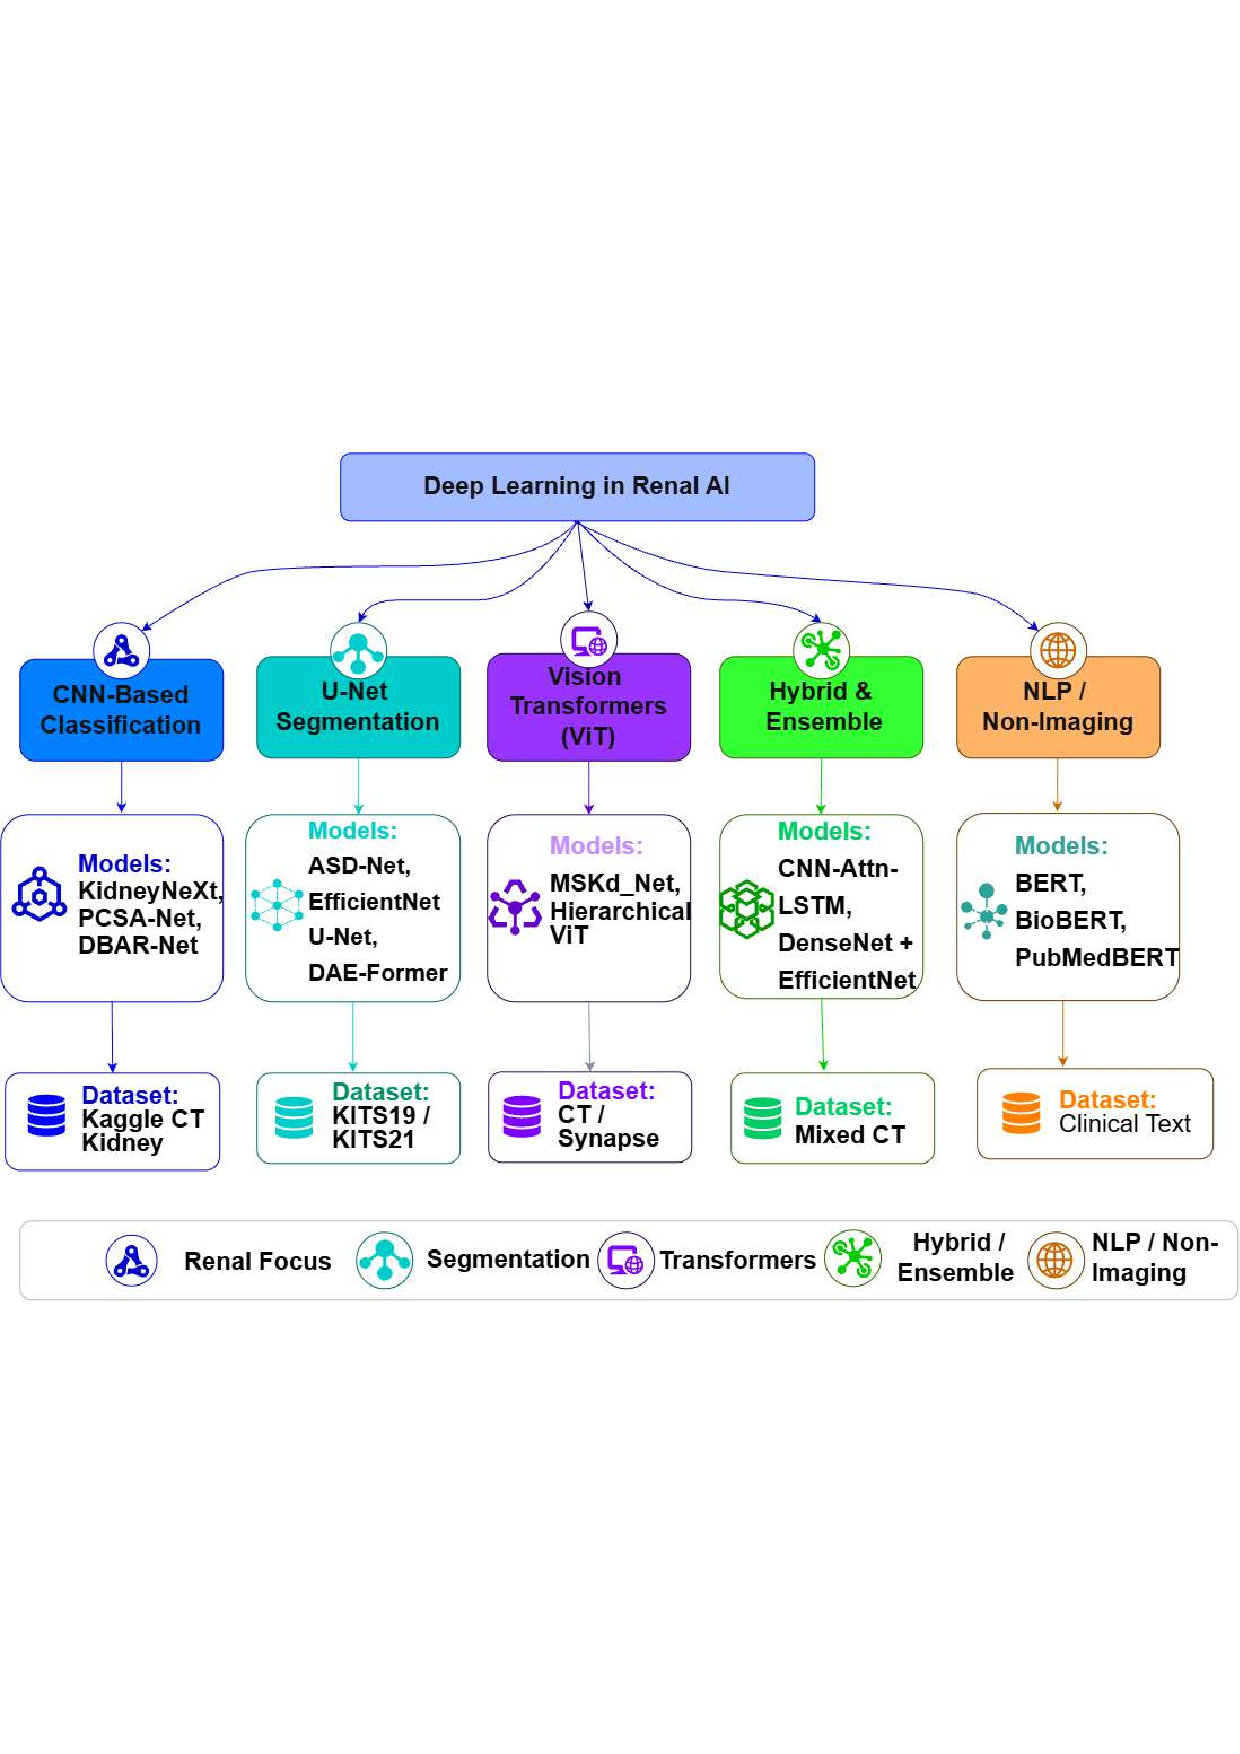
\includegraphics[width=\textwidth]{images/taxonomy_tree.pdf}
\caption{Taxonomy of deep learning architectures utilized in renal disease diagnosis, categorized by foundational feature-extraction mechanisms and their functional application.}
\label{fig:taxonomy}
\end{figure*}

\subsection{Convolutional Neural Networks (CNNs)}
CNNs remain the foundational backbone of medical image analysis due to their inherent translation invariance and efficiency in extracting localized spatial hierarchies. Within renal applications, they are primarily deployed across two functional domains.

\textbf{3D Volumetric Segmentation:} For spatial boundary mapping, the U-Net architecture and its 3D variants have dominated benchmark leaderboards. The symmetric encoder-decoder structure effectively recovers spatial resolution lost during downsampling~\cite{abdelrahman2022deep}. Recent optimizations focus on structurally modifying this core. For instance, the ASD-Net introduces an asymmetric spatial-channel convolution module to better capture irregular tumor boundaries~\cite{ji2024asdnet}, while other frameworks integrate Convolutional Block Attention Modules (CBAM) to suppress background parenchymal noise and highlight critical regions of interest~\cite{gohil2024kidney}.

\textbf{Rapid Triage Classification:} For multi-class classification, lightweight CNNs are prioritized for their high-throughput inference capabilities. Beyond these specialized boundary-mapping networks, numerous studies have successfully deployed traditional, lightweight CNN variants and ensemble methods to establish foundational diagnostic baselines for general renal abnormality detection \cite{alzubi2022kidney, bhandari2023lightweight, rathva2025ensemble, tarul2025empirical, pimpalkar2025fine, abdelrahman2023efficientnet, zhao2023automatic, chen20215d}. Architectures like KidneyNeXt leverage pyramid channel and spatial attention networks to achieve rapid diagnostic triage on standard clinical hardware, efficiently categorizing 2D axial slices into normal, cyst, tumor, or stone classifications~\cite{alqahtani2025kidneynext}.

\subsection{Vision Transformers (ViTs)}
Despite their success, CNNs are fundamentally limited by their localized receptive fields. They struggle to model long-range global dependencies—such as the spatial relationship between a multi-focal renal cell carcinoma and the broader urinary tract. 

\textbf{Global Context Modeling:} Vision Transformers address this limitation by treating images as sequences of flattened patches, applying self-attention mechanisms to weigh the global context of the entire scan simultaneously~\cite{islam2022vision}. Pure attention networks allow the model to understand holistic anatomical relationships.

\textbf{Patch-Based Multi-Scale ViTs:} Frameworks utilizing Swin Transformers attempt to reintroduce a degree of spatial hierarchy into the attention mechanism. However, pure Transformer models remain notoriously data-hungry and computationally expensive, often requiring massive pre-training datasets that are scarce in specialized medical domains. 

\subsection{Hybrid CNN-Transformer Architectures}
To bridge the gap between local precision and global contextual awareness, the current state-of-the-art has converged on Hybrid CNN-Transformer architectures. These models leverage CNN encoders to extract fine-grained, high-resolution local features and utilize Transformer modules to capture global semantic relationships.

\textbf{Cascaded Fusion:} Several notable frameworks highlight this synthesis through sequential processing. The H2Former introduces a cascaded hybrid network that continuously passes CNN and Transformer representations back and forth, achieving superior performance on complex medical image segmentation tasks~\cite{he2023h2former}.

\textbf{Dual Attention \& Routing:} Other architectures focus on optimizing the attention bottleneck. The DAE-Former utilizes a dual attention-guided efficient Transformer to provide multi-organ contouring with highly accurate spatial mapping~\cite{azad2023daeformer}. More recently, architectures like BRAU-Net++ have integrated Bi-Level Routing Attention into a U-shaped topology, significantly reducing the quadratic computational complexity of traditional self-attention while maintaining state-of-the-art Dice scores on renal benchmarks~\cite{lan2024braunet}.

By fusing these modalities, hybrid networks represent the most promising computational foundation for the unified clinical pipelines required in modern nephrology.

% SECTION 5: EXPLAINABILITY (XAI)

\section{Explainability and Clinical Trustworthiness}
\label{sec:xai}

State-of-the-art performance on benchmark datasets does not by itself, justify clinical deployment. As deep learning architectures approach diagnostic parity with specialist radiologists in renal imaging tasks, the central question has shifted from \textit{how accurate?} to \textit{how trustworthy?} Explainable AI (XAI) sits at the heart of this transition: it provides the interpretive scaffolding through which complex model decisions can be audited, validated, and ultimately trusted by the clinicians who act on them. This section examines why transparency is a non-negotiable requirement in nephrology-oriented AI, evaluates the practical landscape of post-hoc visualization and inherently interpretable design, and considers how these tools together support a collaborative, human-in-the-loop clinical workflow.

\subsection{Why Explainability Matters in Surgical Planning}
\label{subsec:why_xai}

High Dice scores and classification accuracies are necessary but insufficient criteria for surgical AI. In nephrology, automated output directly shape high-stakes procedural decisions from preoperative planning for Percutaneous Nephrolithotomy (PCNL) to intraoperative guidance during robot-assisted partial nephrectomies~\cite{li2022automatic}. Under these conditions, an unexplained prediction carries genuine clinical risk: if a model flags a renal mass without indicating which imaging features drove that classification, the clinician has no reliable means to confirm or contest it~\cite{kadhim2024machine}.

This accountability gap is not merely philosophical. A comparative study on stone-free rate prediction demonstrated that large language models, despite their broad linguistic capabilities, failed to outperform validated clinical scoring systems precisely because their reasoning chains were opaque and could not be subjected to clinical scrutiny~\cite{elmaagac2026comparison}. The authors identified non-transparency as a primary barrier to adoption--a finding that generalises across deep learning modalities in urological AI. XAI addresses this by transforming black-box predictions into auditable, spatially grounded justifications, repositioning automated systems as decision-support tools rather than autonomous diagnostic agents.

\subsection{Gradient-Based Visualizations: Grad-CAM and Variants}
\label{subsec:gradcam}

Gradient-weighted Class Activation Mapping (Grad-CAM) remains the most widely adopted post-hoc interpretability technique in renal imaging, owing to its architectural agnosticism and low implementation overhead. By back-projecting the spatial gradients of the final convolutional layer onto the input image, Grad-CAM generates coarse localization heatmaps that identify the anatomical regions most influential to a given prediction. In CT-based renal analysis, this mechanism offers clinicians a rapid visual sanity check: does the model's activation align with the pathological region, or is it responding to irrelevant background structure?

Multi-center 3D CNN frameworks have leveraged these maps to establish explainable visual correlations between lesion size and detection confidence across heterogeneous imaging protocols~\cite{liang2025multicenter}. Attention-augmented detectors similarly employ spatial and channel attention outputs to confirm that network focus concentrates on calcified stone deposits or irregular tumor margins rather than adjacent parenchymal tissue~\cite{sajid2026yolov8}. The DAE-Former architecture goes a step further, demonstrating that Transformer-based attention maps can be inherently gradient-interpretable, providing multi-organ contouring outputs with built-in spatial accountability for radiation dose planning~\cite{azad2023daeformer}.

Nonetheless, gradient-based explanations carry well-documented limitations. Their spatial resolution is constrained by the receptive field of the final convolutional stage, and they are susceptible to highlighting imaging features that are statistically correlated with the target class without being causally responsible for the pathology. This distinction---correlation versus causation in saliency mapping---remains an open research problem and motivates the exploration of more structurally integrated interpretability approaches.


\subsection{Inherent Interpretability vs.\ Post-Hoc Analysis}
\label{subsec:inherent_vs_posthoc}

Post-hoc methods like Grad-CAM and SHAP (SHapley Additive exPlanations) offer broad applicability across pre-trained networks, but their explanations are approximations of decisions already made. A fundamentally different design philosophy embeds interpretability into the architecture itself, ensuring that the reasoning process is transparent by construction rather than reconstructed after the fact.

Convolutional Block Attention Modules (CBAM) and Bi-Level Routing Attention (BRA), as deployed in hybrid CNN-Transformer segmentation networks, produce explicit spatial focus matrices at each feature extraction stage~\cite{lan2024braunet}. The practical implication is that a radiologist reviewing such a model's output can trace exactly which spatial regions were weighted at each processing layer, rather than relying on a single terminal heatmap. This architectural transparency is particularly valuable in multi-class scenarios: in the CNN-Attention-LSTM framework for sequential kidney stone detection, the integrated attention outputs identify high-activation stone positions slice-by-slice, constructing an auditable diagnostic chain across volumetric CT series~\cite{alebada2026hybrid}.

At the other end of the interpretability spectrum, classical feature engineering approaches---such as Gray-Level Co-occurrence Matrix (GLCM) texture analysis combined with statistical feature selection (POE+ACC)---offer fully deterministic, rule-based transparency~\cite{farjad2021ct}. This drive for architectural transparency, alternative structured feature extraction, and domain-adapted text-vision models is similarly documented across a wide swath of earlier computational frameworks and hybrid benchmarks~\cite{hossain2024adaptive, elton2022deep, lee2020biobert, fang2023bioformer, luo2022biogpt, hatsutani2023protuberance, sharma2025hybrid, martin2025evaluation}. These methods produce inherently interpretable decision boundaries but sacrifice the semantic depth and contextual sensitivity that deep representations provide. In practice, neither extreme is universally optimal; the appropriate balance depends on the clinical task, the regulatory environment, and the degree of radiologist oversight available. Hybrid approaches that pair deep visual features with structured, interpretable output heads represent the most pragmatic direction for near-term clinical deployment.

\subsection{Human-AI Collaboration and Standardisation}
\label{subsec:human_ai}

The practical goal of XAI in renal diagnostics is not to make every model decision comprehensible in isolation, but to calibrate how much autonomy clinicians should delegate to automated systems across different task types. For routine multi-class triage on standard CT protocols, a well-validated model with Grad-CAM outputs may provide sufficient transparency. For edge cases---atypical tumor morphologies, multi-component calculi, or post-operative anatomy---clinician override supported by detailed attention maps becomes essential.

Embedding XAI into the clinical workflow shifts the radiologist's role from exhaustive manual screening to targeted validation of AI-highlighted anomalies~\cite{abdelrahman2022deep}. This redistribution of cognitive load is clinically meaningful: it reduces interpretation fatigue in high-volume imaging centres while preserving the specialist judgment that automated systems cannot yet replicate. The limiting factor is not technical capability but the absence of standardised interpretability protocols. As a systematic review of hybrid CNN-Transformer models across 112 studies confirmed, most architectures are evaluated without consistent XAI benchmarks, making cross-study comparison of trustworthiness claims difficult~\cite{papanastasiou2024systematic}. Emerging frameworks such as Causal Representation Learning (CRL) offer a principled route toward standardisation by formalising the causal reasoning that links imaging features to clinical outcomes, though their integration into production medical AI pipelines remains an active area of development.


% SECTION 6: FUTURE DIRECTIONS (UNIFIED FRAMEWORK)

\section{A Proposed Unified Clinical Framework}
\label{sec:framework}

The preceding sections have documented substantial progress across individual diagnostic tasks---classification, segmentation, NLP, and interpretability---yet the practical gap between algorithmic benchmarks and operational clinical tools remains wide. This section pivots from retrospective synthesis to a prospective architectural proposal. Serving as a roadmap for future researchers, this proposed pipeline is a conceptual synthesis of the best-performing models identified in Section~\ref{sec:architectures}. We introduce a theoretical three-stage multimodal framework designed to unify renal triage, surgical boundary mapping, and automated clinical reporting within a single coherent pipeline, culminating in an interactive dashboard that addresses both the computational and workflow demands of active nephrological practice.

% ------------------------------------------
\subsection{The Three-Stage Clinical Gap}
\label{subsec:clinical_gap}

The fragmentation of current renal AI is not merely a modelling limitation---it reflects a systemic disconnect in how the field has framed the clinical problem. Classification networks are optimised for category discrimination; segmentation models for spatial precision; NLP systems for unstructured text. None of these, individually, addresses the full diagnostic cycle that a nephrologist must navigate: \textit{What is the pathology? Where exactly are its margins? And what does the patient's clinical history tell us about management?}

A model that achieves 99\% accuracy on the Kaggle CT Kidney dataset~\cite{ahmed2021ct} provides no direct guidance on whether a 2.8~cm renal mass requires immediate surgical intervention or active surveillance. Conversely, a highly accurate volumetric segmentation model for the KiTS challenges~\cite{heller2023kits21} produces surgical masks without the accompanying multi-class discrimination needed to guide pre-operative planning for heterogeneous pathologies. These isolated strengths, when combined with the lack of native integration with patient health records, produce a workflow that demands substantial radiologist synthesis---precisely the burden that clinical AI should reduce. The conceptual framework proposed here (Figure~\ref{fig:framework}) explicitly targets this translational gap by treating detection, surgical mapping, and automated reporting as dependent, sequentially coupled stages rather than independent computational problems.

\begin{figure*}[htbp]
\centering
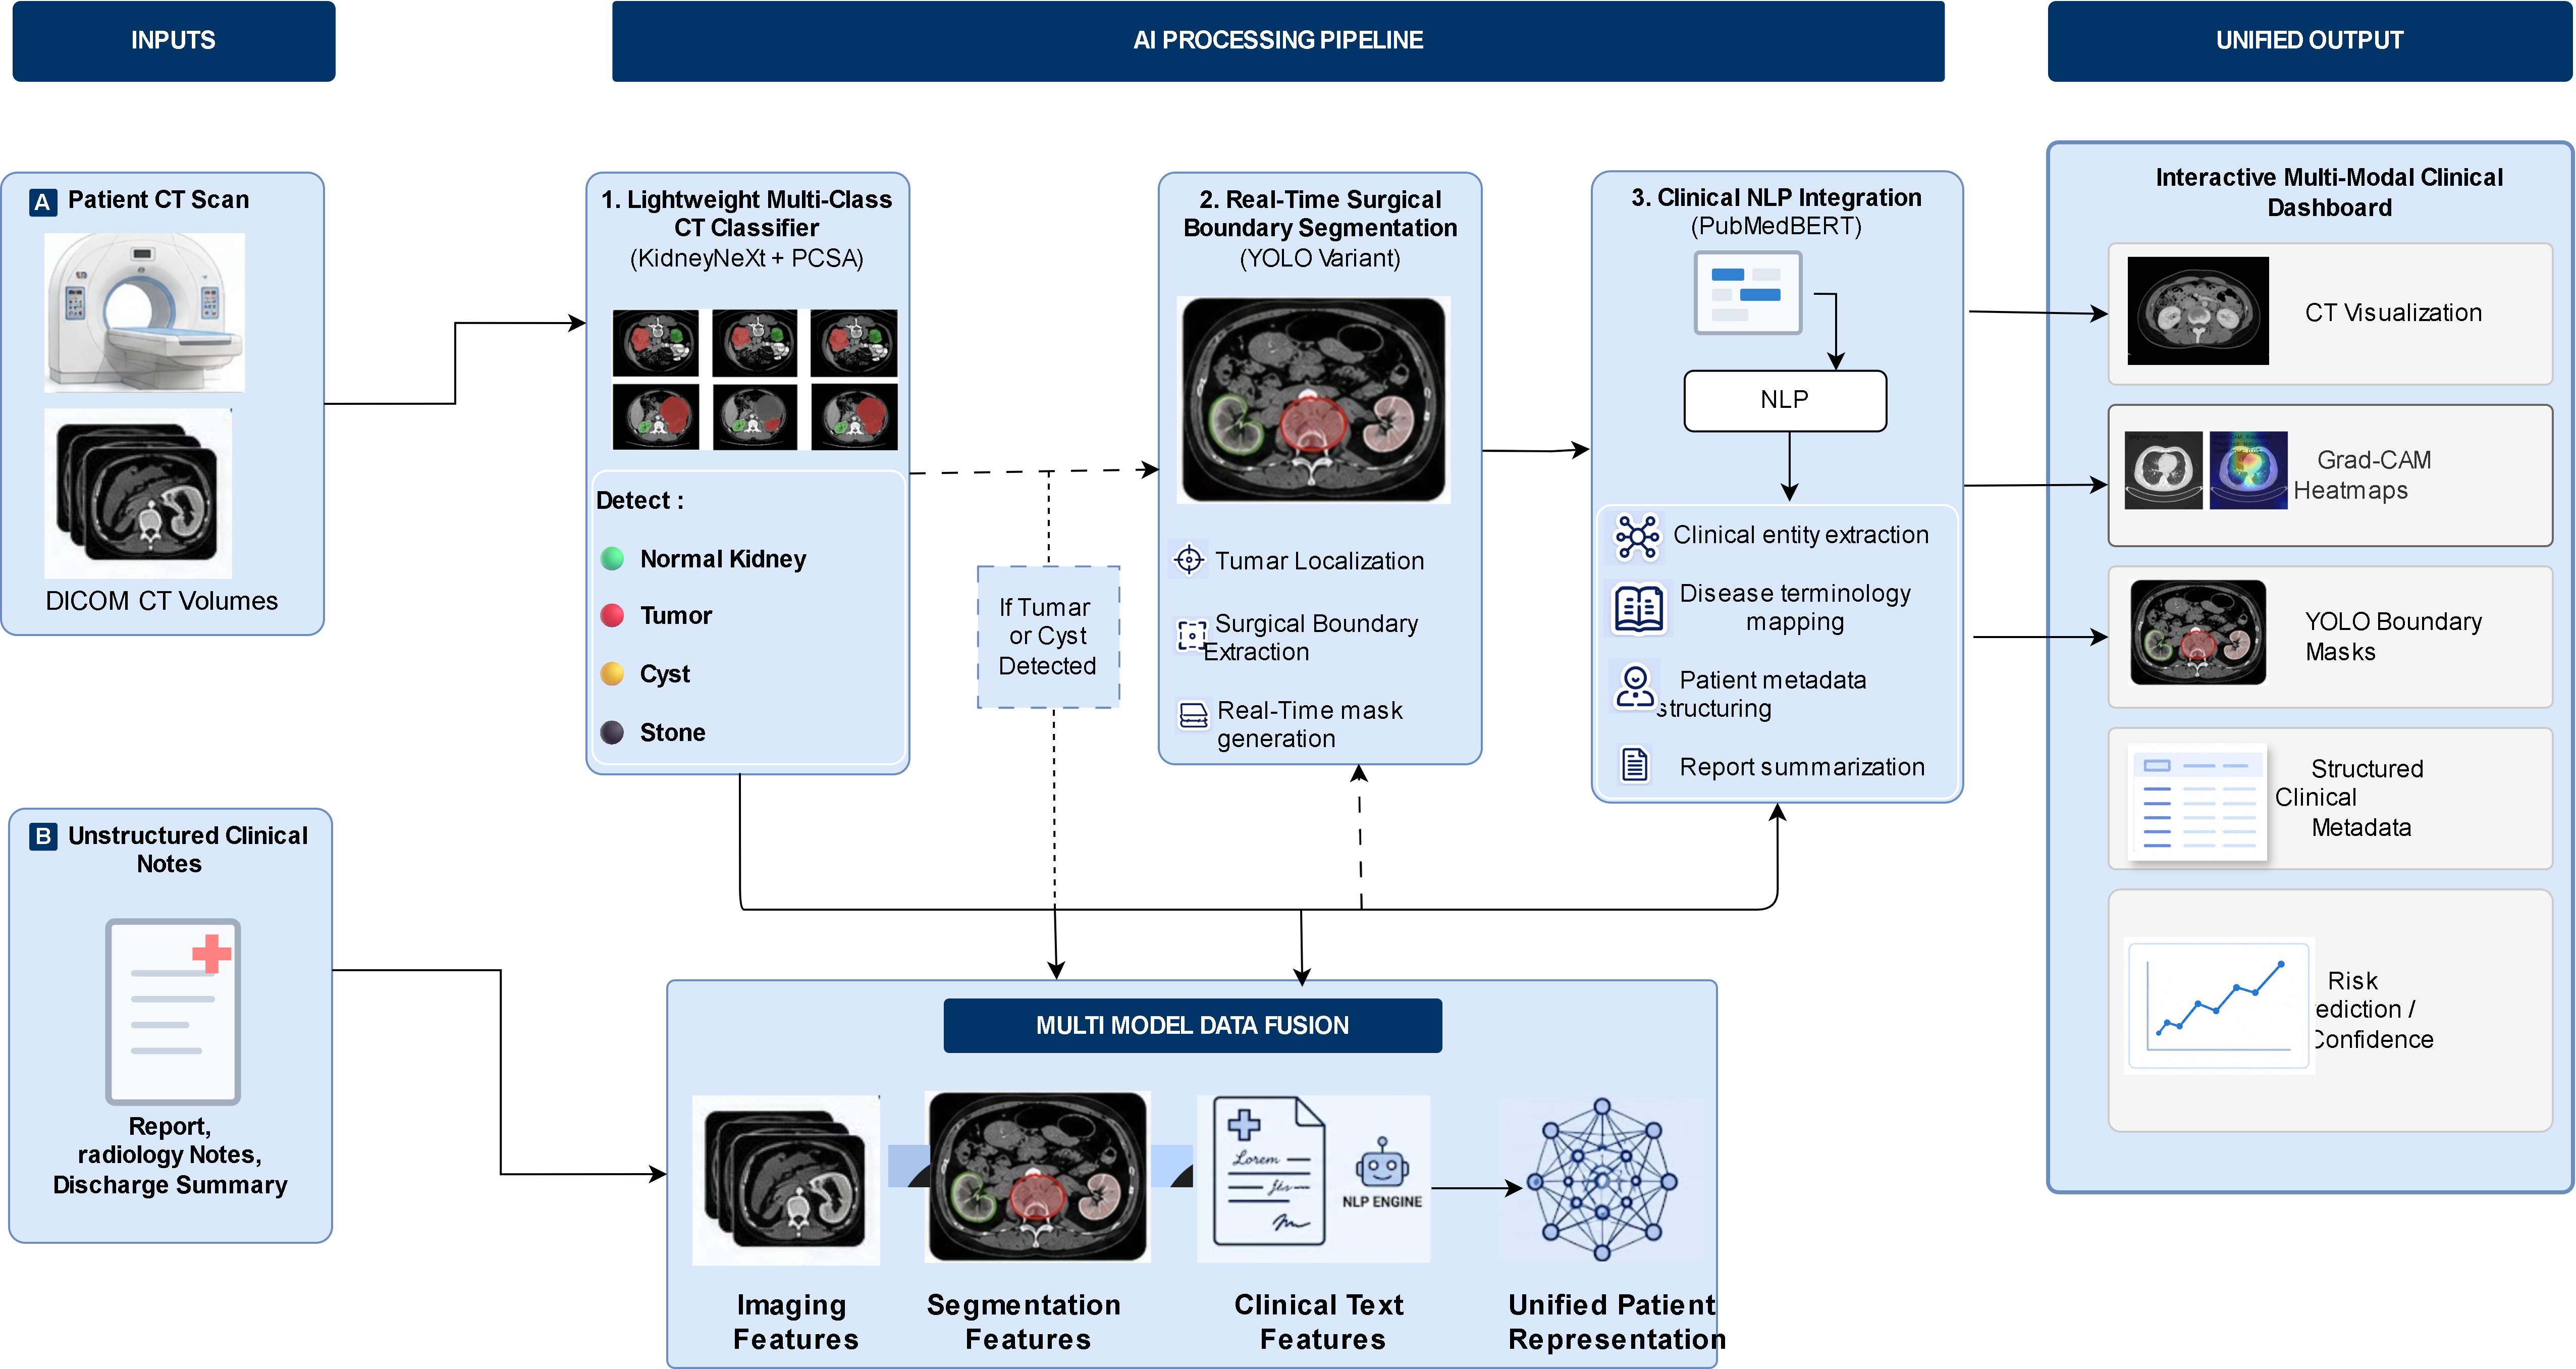
\includegraphics[width=\textwidth]{images/pipeline.png}
\caption{\textbf{Proposed Unified Clinical Pipeline.} The theoretical three-stage multimodal framework integrates lightweight CT classification for rapid triage (Stage~1), YOLO-based real-time boundary segmentation triggered by critical findings (Stage~2), and PubMedBERT-driven clinical NLP for automated report generation (Stage~3). All outputs converge in an interactive clinical dashboard.}
\label{fig:framework}
\end{figure*}

\subsection{Stage 1: Automated Renal Pathology Classification}
\label{subsec:stage1_classification}

The first stage functions as a high-throughput triage gate. Hospital Picture Archiving and Communication Systems (PACS) process substantial daily imaging volumes, and the practical viability of any AI-assisted workflow depends on architectures lightweight enough to operate within standard clinical computational budgets. Drawing on the KidneyNeXt backbone augmented with Pyramid Channel and Spatial Attention (PCSA) modules~\cite{alqahtani2025kidneynext, tawfik2026pcsa}, this stage would theoretically perform rapid multi-class categorisation based on the benchmark capabilities of these architectures across the four clinically relevant renal pathology categories---normal parenchyma, complex cysts, calcified stones, and solid malignancies---on standard 12,446-image CT datasets. 

Critically, this classification stage is not an end-point but a gating mechanism. Normal findings are logged and discharged from further processing; critical findings---tumour or obstructing calculus detections---conditionally route the imaging data to Stage~2. This conditional architecture ensures that computationally expensive segmentation resources are deployed selectively, preserving system throughput without sacrificing diagnostic coverage.

\subsection{Stage 2: Real-Time Surgical Boundary Segmentation}
\label{subsec:stage2_segmentation}

Preoperative planning for robot-assisted partial nephrectomy or PCNL demands spatial precision that extends well beyond what classification outputs provide. Surgeons require exact tumour margins, stone dimensions, and proximity to collecting system structures to minimise parenchymal sacrifice and reduce vascular complication risk. This stage addresses that need through real-time instance segmentation, proposing YOLOv11-based architectures adapted for medical imaging~\cite{akhtar2026yolov11}.

The case for a YOLO-family approach over traditional 3D U-Nets rests on practical clinical deployment constraints. While architectures such as ASD-Net~\cite{ji2024asdnet} or the spatial-channel attention enhanced U-Net~\cite{gohil2024kidney} deliver strong Dice performance on KiTS benchmarks, their 3D volumetric convolutions introduce inference latencies that are incompatible with real-time surgical guidance. A streamlined single-stage detector, operating on axial CT slices with CBAM-augmented attention, translates bounding box predictions into actionable surgical boundary masks at frame rates appropriate for intraoperative use, delivering the low-latency spatial feedback that the clinical environment demands.

\subsection{Stage 3: Clinical NLP Integration}
\label{subsec:stage3_nlp}

The third stage addresses a dimension of clinical AI that the imaging literature has largely treated as peripheral: the structured representation of unstructured clinical knowledge. Radiological reports, referring physician notes, and laboratory results contain contextual information---prior stone episodes, family history of renal cell carcinoma, eGFR trajectories---that no amount of CT pixel analysis can replicate. Integrating this textual context into the diagnostic workflow requires domain-adapted biomedical language models.

By deploying PubMedBERT~\cite{gu2021domain} fine-tuned for clinical Named Entity Recognition (NER), this stage would theoretically ingest the unstructured patient health record alongside the visual metadata produced in Stages~1 and~2. The NLP engine extracts structured clinical entities---pathology type, anatomical location, relevant comorbidities, and urgency indicators---and maps them against the imaging findings. A confirmed 3~cm lower-pole renal mass, when cross-referenced with a clinical note documenting haematuria and elevated creatinine, yields a materially different management recommendation than the same imaging finding in an asymptomatic screening context. This multimodal synthesis is precisely the integration that current literature identifies as absent from deployed renal AI systems~\cite{sreenivas2025enhancing}.

\subsection{The Integrated Clinical Dashboard}
\label{subsec:unified_dashboard}

The technical outputs of the three stages described above are clinically meaningful only if they are accessible and interpretable at the point of care. The proposed dashboard consolidates four information streams into a single interface: the original DICOM CT slice; the Grad-CAM interpretability overlay from Stage~1; the YOLO-generated surgical boundary masks from Stage~2; and the structured clinical metadata compiled by Stage~3. This co-presentation is deliberate---it enables the reviewing nephrologist or urologist to cross-validate the automated findings against the original imaging and the patient's clinical context without navigating multiple systems.

The design principle underlying this dashboard is epistemic transparency: every automated output is accompanied by its visual justification, and the clinician retains final authority at each decision point. This architecture directly addresses the accountability concerns raised in Section~\ref{sec:xai}, embedding XAI not as a post-development afterthought but as a structural component of the clinical interface. Integration with HL7 FHIR standards ensures that dashboard outputs feed directly into existing hospital information systems, avoiding the manual transcription overhead that represents one of the most persistent barriers to AI adoption in clinical settings~\cite{liang2025multicenter}.

% SECTION 7: REAL-WORLD DEPLOYMENT CHALLENGES

\section{Real-World Deployment Challenges}
\label{sec:challenges}

Demonstrating strong performance on curated benchmark datasets is a necessary but insufficient condition for clinical deployment. The gap between a model that achieves 99\% accuracy on the Kaggle CT Kidney dataset and one that functions reliably across the heterogeneous conditions of a busy district general hospital is substantial, and the literature has only recently begun to address it systematically. This section examines the three most consequential barriers: distributional generalisation, the mismatch between algorithmic and clinical metrics, and the engineering complexity of PACS integration.

\subsection{Data Generalisation and Modality Shifts}
\label{subsec:generalization_shifts}

The majority of high-performing renal AI models are trained and validated on a small number of well-curated repositories. The Kaggle CT Kidney dataset~\cite{ahmed2021ct, hossain2025detection} and the KiTS challenge cohorts~\cite{heller2023kits21} have been invaluable for establishing algorithmic baselines, but their controlled acquisition conditions do not reflect the scanner heterogeneity encountered in routine clinical imaging. Slice thickness, reconstruction kernel, contrast phase, and vendor-specific HU calibration all vary substantially across institutions, and these variations systematically degrade model performance in ways that benchmark evaluations do not capture~\cite{abdelrahman2022deep}. 

This reliance on homogeneous training data or single-modality captures is a prevalent limitation observed across a broad spectrum of current multi-task, super-resolution, and volumetric segmentation literature~\cite{abdalla2025axial, ma2022flare, macin2025kidneynext, xie2020seru, nguyen2025super, gao2026multitask, chen2023glunet, sherryl2022ied}.

The multi-phase nature of renal CT protocols compounds this problem. Models trained primarily on portal venous or nephrographic phase acquisitions frequently fail on non-contrast studies, where calculi are most visible but soft-tissue contrast is limited, and on arterial phase acquisitions, where vascular anatomy introduces confounding HU patterns~\cite{liang2025multicenter, ye2026automated}. Without prospective multi-centre validation incorporating the full range of acquisition protocols encountered in clinical practice, published performance figures should be interpreted with caution. The models reviewed in this survey that explicitly report external validation---notably the multi-centre 3D CNN of Liang et al.~\cite{liang2025multicenter} and the DBAR-Net of Sharon and Anbarasi~\cite{sharon2025attention}---represent the direction that the field must move, but they remain the exception rather than the rule.

\subsection{Algorithmic vs.\ Clinical Metrics}
\label{subsec:metrics_gap}

The standard performance vocabulary of deep learning---Dice Similarity Coefficient, Intersection over Union, macro F1-score---was designed to measure spatial or categorical alignment between model outputs and annotated ground truth. These metrics are well-suited to comparing architectures on a fixed dataset, but they are poor proxies for the outcomes that matter clinically.

Consider a model that achieves a Dice score of 0.92 on kidney tumour segmentation. That figure may reflect near-perfect delineation of a large, well-defined clear cell carcinoma while entirely missing a 4~mm satellite lesion at the tumour margin---a miss that has negligible impact on the aggregate score but significant implications for resection completeness~\cite{raj2022deep, gohil2024kidney}. Equally, a stone detection model reporting 96\% accuracy may perform adequately on stones larger than 5~mm while failing on sub-3~mm calculi that are clinically relevant for PCNL access planning~\cite{ye2026automated}. The disconnect is systematic: optimising for pixel-level metrics during training does not guarantee that the resulting model behaviour aligns with surgical priorities.

Addressing this requires a fundamental shift in how renal AI is evaluated. Clinical validation studies should incorporate task-specific metrics: stone-free rate prediction, surgical margin clearance rates, reduction in time-to-report, and inter-observer variability across radiologist cohorts~\cite{noorelahi2025pacs}. Progress in this direction is slow---partly because such endpoints require prospective clinical trial infrastructure---but it is a prerequisite for regulatory approval and sustainable clinical adoption.

\subsection{PACS Integration and Computational Overhead}
\label{subsec:pacs_integration}

Even a model that satisfies both generalisation and clinical validity requirements faces a third class of challenge: the practical engineering of integration into legacy hospital infrastructure. Most deployed clinical imaging systems were not designed with deep learning inference in mind, and retrofitting AI processing into existing PACS workflows introduces non-trivial latency, data governance, and interoperability constraints.

Large-scale 3D architectures---volumetric U-Net variants, multi-scale Vision Transformers---typically require enterprise-grade GPU hardware (e.g., NVIDIA A100 or Tesla-class accelerators) to maintain inference speeds compatible with clinical workflows~\cite{azad2023daeformer, li2022automatic}. The majority of district-level clinical environments lack this infrastructure, and even where it exists, the overhead of routing DICOM data to GPU-equipped inference servers introduces latency that may be unacceptable for time-sensitive applications such as emergency renal colic triage~\cite{ye2026automated}. Model compression techniques---quantisation, knowledge distillation, and pruning---offer partial mitigation, but their application to medical imaging models requires careful validation to ensure that compression does not disproportionately degrade performance on the rare but clinically critical edge cases~\cite{kadhim2024machine}.

Interoperability presents a parallel challenge. Clinical AI outputs must be delivered in formats that integrate natively with hospital information systems and downstream documentation workflows. The HL7 FHIR standard provides a structured mechanism for this integration, and its adoption by frameworks such as the multi-centre urinary disease detection system of Liang et al.~\cite{liang2025multicenter} demonstrates that PACS-compatible deployment is achievable. Scaling this approach across diverse institutional environments, each with different legacy system configurations, nonetheless remains a substantial engineering undertaking that the research community has yet to address systematically~\cite{ali2024comprehensive}.

% SECTION 8: CONCLUSION


\section{Conclusion}
\label{sec:conclusion}


\subsection{Summary of Findings}
\label{subsec:summary}

This survey has traced the progression of deep learning in renal imaging from early CNN-based multi-class classifiers through to the current generation of hybrid Vision Transformer and attention-augmented architectures. Several clear trajectories emerge from the literature. First, raw classification and segmentation accuracy---while still improving---is no longer the primary differentiator between architectures; the field is increasingly stratified by computational efficiency, architectural interpretability, and demonstrated robustness to domain shift. Second, the adoption of Explainable AI has moved from optional enhancement to practical necessity: models deployed in surgical planning contexts without transparent decision mechanisms face significant barriers to clinical acceptance, regardless of their benchmark performance. Third, and most significantly, the prevailing model-centric framing of renal AI---in which each architecture is evaluated in isolation on a static dataset---is increasingly misaligned with the integrated, multimodal nature of actual clinical workflows.

The reviewed literature also reveals persistent structural gaps. Multi-centre external validation remains rare. Clinical outcome metrics are seldom reported alongside algorithmic ones. NLP integration with imaging pipelines is largely theoretical in existing publications. These gaps are not incidental; they reflect the boundary between what is tractable as a machine learning problem and what is required for clinical translation.

\subsection{Clinical Outlook}
\label{subsec:outlook}

The trajectory of renal AI points unambiguously toward multimodal integration. The isolated successes documented across classification, segmentation, and language modelling are necessary precursors, but they become clinically transformative only when composed into coherent diagnostic pipelines. The unified framework proposed in Section~\ref{sec:framework} represents one such composition: a sequentially coupled system in which lightweight classification gates downstream segmentation, segmentation outputs inform report generation, and all findings are presented through an interpretable, PACS-integrated interface.

Realising this vision requires progress on multiple fronts simultaneously---generalisation, evaluation methodology, and systems engineering---none of which can be solved by algorithmic innovation alone. It demands prospective clinical collaborations, standardised benchmarking protocols, and regulatory frameworks adapted to the iterative nature of deployed AI. The role of the nephrologist and urologist in this process is not diminished by automation; it is recentred. Human clinical judgment remains the validating authority for AI outputs, and designing systems that honour that authority---through transparency, appropriate uncertainty communication, and genuine human override capacity---is the most consequential design challenge facing renal AI today.

\section*{Declarations}

\textbf{Funding}: The authors declare that no funds, grants, or other support were received during the preparation of this manuscript.

\textbf{Conflict of interest/Competing interests}: The authors declare that they have no conflict of interest or competing interests relevant to this study.

\textbf{Ethics approval}: Not applicable (this study is a comprehensive systematic review of published literature and does not involve animal or human clinical trials conducted by the authors).

\textbf{Consent to participate}: Not applicable.

\textbf{Consent for publication}: Not applicable.

\textbf{Data availability}: All benchmark datasets discussed and summarized in this review (e.g., KiTS19, KiTS21, Kaggle CT Kidney Dataset, FLARE, Synapse) are publicly accessible via the respective repository links and challenge portals cited in Table~\ref{tab:datasets}.

\textbf{Code availability}: Not applicable.

\textbf{Author contributions}: All authors contributed significantly to this work. Conceptualization, methodology, and literature synthesis were performed by Atharv Ashwin Chavan, Yash Sagar Kumbhoje, Pradnya Ravindra Shikalgar, and Kanishka Subhash Gavali under the academic supervision and guidance of Prof. Mrs. Gautami G. Shingan. The initial draft of the manuscript was compiled by Atharv Ashwin Chavan and Yash Sagar Kumbhoje. Critical review and formal editing were contributed by all authors. All authors reviewed and approved the final manuscript.

%%===========================================================================================%%
%% Bibliography                                                                              %%
%%===========================================================================================%%

\bibliography{references}

\end{document}
